\documentclass[12pt, a4paper]{article}

% --- PREAMBUŁA (ustawienia dokumentu) ---
\usepackage[utf8]{inputenc}       % Kodowanie znaków
\usepackage[T1]{fontenc}          % Polskie znaki (ą, ć, ę, ł, ń, ó, ś, ź, ż)
\usepackage[polish]{babel}        % Polskie reguły dzielenia wyrazów i nazwy (np. "Spis treści")
\usepackage{amsmath}              % Pakiety matematyczne (niezbędne do macierzy)
\usepackage{amsfonts}             % Czcionki matematyczne
\usepackage{amssymb}              % Symbole matematyczne (np. nieskończoność)
\usepackage{geometry}             % Ustawienia marginesów
\usepackage{csvsimple}
\usepackage{float}
\usepackage{graphicx}
\usepackage{siunitx}
\usepackage{booktabs} % Wymagane przez pandas.to_latex()
\usepackage{textcomp} % Dla symbolu mikrona

\geometry{
	a4paper,
	left=2.5cm,
	right=2.5cm,
	top=2.5cm,
	bottom=2.5cm
}
\usepackage{indentfirst}          % Wcięcia w pierwszych akapitach
\usepackage{hyperref}             % Aktywne odnośniki w dokumencie
\usepackage{setspace}             % Interlinia
\setstretch{1.35}                 % ZWIĘKSZONA INTERLINIA (ok. 1.5 linii)
\setlength{\parskip}{0.5em}       % Dodatkowy odstęp między akapitami
\usepackage{csvsimple}
\usepackage{booktabs} % Dla ładniejszych linii \toprule, \midrule, \bottomrule

% --- DANE DO STRONY TYTUŁOWEJ ---
\title{\textbf{Sprawozdanie z projektu nr 2} \\ \large Asymetryczny Problem Komiwojażera (ATSP)
	\\ \large Projektowanie Efektywnych algorytmów}
\author{Karol Gąsior / 280913}
\date{\today} 

%\usepackage[polish]{cleveref}
% --- POCZĄTEK WŁAŚCIWEGO DOKUMENTU ---
\begin{document}
	
	\maketitle % Generuje tytuł, autora i datę
	\newpage
	\tableofcontents % Automatyczny spis treści
	\newpage
	
	\section{Wstęp teoretyczny}
	
	\subsection{Algorytm podziału i ograniczeń (Branch and Bound)}
	W ramach drugiego etapu projektu zaimplementowano algorytm podziału i ograniczeń (ang. \textit{Branch and Bound}, B\&B) w celu rozwiązania asymetrycznego problemu komiwojażera (ATSP). Metoda ta jest dokładnym algorytmem optymalizacyjnym, który w przeciwieństwie do przeglądu zupełnego nie sprawdza każdej możliwej permutacji w sposób naiwny. 
	
	Działanie algorytmu opiera się na budowaniu drzewa przestrzeni rozwiązań. W każdym węźle drzewa obliczane jest tzw. dolne ograniczenie (ang. \textit{Lower Bound}, LB) kosztu dla wszystkich ścieżek wychodzących z danego węzła. Jeżeli wartość LB danej gałęzi przekracza lub jest równa kosztowi najlepszego dotychczas znalezionego rozwiązania (górne ograniczenie), cała gałąź jest odrzucana (odcinana). Zgodnie z założeniami projektowymi, algorytm został wyposażony w trzy metody przeglądania tak zbudowanej przestrzeni: \textit{breadth-first-search} (przeszukiwanie wszerz), \textit{depth-first-search} (przeszukiwanie w głąb) oraz \textit{lowest-cost} (najlepszy najpierw).
	
	% ---------------------------------------------------------------------------------------------------------------------
	
	\section{Przykład praktyczny algorytmu B\&B (Depth-First Search) dla $N=3$}
	
	Poniżej przedstawiono działanie algorytmu krok po kroku dla przykładowej instancji problemu o małej wartości $N$. Przyjęto strategię przeszukiwania w głąb (DFS), a dolne ograniczenie wyznaczane jest metodą Little'a. Niech początkowa asymetryczna macierz kosztów $M$ wynosi:
	
	$$ M = \begin{bmatrix} \infty & 10 & 15 \\ 5 & \infty & 9 \\ 6 & 12 & \infty \end{bmatrix} $$
	
	\textbf{Krok 1: Węzeł początkowy (Root) i wyznaczenie LB}
	\begin{itemize}
		\item \textbf{Redukcja wierszy:} W każdym wierszu znajdujemy wartość minimalną i odejmujemy ją od pozostałych elementów wiersza. 
		Minimum wiersza 0: $10$. Po odjęciu: $[\infty, 0, 5]$.
		Minimum wiersza 1: $5$. Po odjęciu: $[0, \infty, 4]$.
		Minimum wiersza 2: $6$. Po odjęciu: $[0, 6, \infty]$.
		Suma redukcji wierszy: $10 + 5 + 6 = 21$.
		\item \textbf{Redukcja kolumn:} Analogicznie odejmujemy minima z kolumn (dla zredukowanej już macierzy).
		Minimum kolumny 0: $0$.
		Minimum kolumny 1: $0$.
		Minimum kolumny 2: $4$. Po odjęciu: kolumna 2 to $[1, 0, \infty]$.
		Suma redukcji kolumn: $0 + 0 + 4 = 4$.
		\item \textbf{Macierz zredukowana węzła początkowego $M'$:}
		$$ M' = \begin{bmatrix} \infty & 0 & 1 \\ 0 & \infty & 0 \\ 0 & 6 & \infty \end{bmatrix} $$
		\item \textbf{Koszt węzła (LB):} $21 + 4 = 25$. Węzeł trafia na \texttt{Stack}.
	\end{itemize}
	
	\textbf{Krok 2: Rozgałęzienie (Branching) z wierzchołka 0}
	Pobieramy węzeł ze stosu. Możemy udać się do miasta 1 lub 2. Zgodnie z metodą DFS, badamy obydwie opcje i umieszczamy je na stosie.
	
	\textit{Węzeł Dziecko A (ścieżka 0 $\rightarrow$ 1):}
	\begin{itemize}
		\item Kopiujemy macierz $M'$. Blokujemy wiersz 0 i kolumnę 1 (ustawiamy na $\infty$). Blokujemy powrót (ustawiamy $M'[1][0] = \infty$).
		\item Macierz przed ponowną redukcją:
		$$ M_A = \begin{bmatrix} \infty & \infty & \infty \\ \infty & \infty & 0 \\ 0 & \infty & \infty \end{bmatrix} $$
		\item Macierz jest już w pełni zredukowana (w każdym niezablokowanym wierszu i kolumnie jest zero). Koszt redukcji $= 0$.
		\item Nowe $LB_A$ = $LB_{poprzednie}$ (25) + Koszt przejścia $M'[0][1]$ (0) + Koszt redukcji (0) = 25.
	\end{itemize}
	
	\textit{Węzeł Dziecko B (ścieżka 0 $\rightarrow$ 2):}
	\begin{itemize}
		\item Blokujemy wiersz 0, kolumnę 2 oraz powrót $M'[2][0]$.
		\item Macierz przed redukcją:
		$$ M_B = \begin{bmatrix} \infty & \infty & \infty \\ 0 & \infty & \infty \\ \infty & 6 & \infty \end{bmatrix} $$
		\item Redukcja wiersza 2 (minimum to 6). Po odjęciu wiersz 2 to $[\infty, 0, \infty]$. Suma redukcji $= 6$.
		\item Nowe $LB_B$ = $LB_{poprzednie}$ (25) + Koszt przejścia $M'[0][2]$ (1) + Koszt redukcji (6) = 32.
	\end{itemize}
	\textbf{Zarządzanie stosem:} Na stos (LIFO) odkładamy Węzeł B, a następnie Węzeł A.
	
	\textbf{Krok 3: Eksploracja DFS (Węzeł A)}
	\begin{itemize}
		\item Ściągamy ze stosu Węzeł A (ścieżka: 0 $\rightarrow$ 1, LB = 25). Ponieważ nie odwiedzono jeszcze wszystkich miast, generujemy jedyne możliwe dziecko: ścieżkę 0 $\rightarrow$ 1 $\rightarrow$ 2.
		\item Macierz zostaje całkowicie wyzerowana/zablokowana, koszt nie rośnie. Kompletna trasa to 0 $\rightarrow$ 1 $\rightarrow$ 2 $\rightarrow$ 0.
		\item Ustawiamy najlepszy dotychczasowy koszt rozwiązania (\textit{upper bound}) na 25.
	\end{itemize}
	
	\textbf{Krok 4: Próba eksploracji Węzła B i odcięcie (Pruning)}
	\begin{itemize}
		\item Ściągamy ze stosu Węzeł B (ścieżka 0 $\rightarrow$ 2, LB = 32).
		\item Ponieważ $LB_B$ (32) jest większe niż dotychczas znalezione najlepsze rozwiązanie (25), algorytm natychmiast odrzuca tę gałąź bez dalszej eksploracji. Stos jest pusty, algorytm kończy działanie.
	\end{itemize}
	
	% ---------------------------------------------------------------------------------------------------------------------
	
	\section{Opis implementacji algorytmu i zastosowanych struktur}
	
	Implementacji dokonano w języku C++ z zachowaniem obiektowego paradygmatu programowania. Mając na uwadze optymalizację pamięciową, wszystkie używane struktury danych są alokowane dynamicznie i zależą wyłącznie od aktualnie wprowadzonego rozmiaru problemu.
	
\subsection{Kluczowe struktury danych}

Efektywność zaimplementowanego algorytmu Branch and Bound opiera się na dekompozycji problemu na niezależne moduły zarządzające stanem węzłów oraz strukturami sterującymi przepływem danych. W projekcie wykorzystano następujące komponenty:

\begin{itemize}
	\item \textbf{Klasa \texttt{Node}:} Stanowi atomowy element drzewa rozwiązań. Każdy obiekt przechowuje dynamicznie alokowaną macierz kosztów (stan po redukcji), bieżący koszt dolnego ograniczenia (\textit{lower bound}), aktualną ścieżkę oraz poziom zagłębienia. Przechowywanie pełnej macierzy w każdym węźle, choć zwiększa narzut pamięciowy, eliminuje konieczność kosztownego operowania na mechanizmach \textit{backtrackingu} i pozwala na pełną izolację stanów podczas eksploracji różnych gałęzi.
	
	\item \textbf{Struktury składujące węzły :} 
	Zaimplementowano trzy odrębne kontenery zarządzające kolejnością odwiedzanych węzłów, co umożliwiło bezpośrednie porównanie strategii przeszukiwania:
	\begin{itemize}
		\item \textbf{Stos (\texttt{NodeStack}):} Wykorzystany w strategii DFS. Pozwala na natychmiastowe dojście do liści drzewa, co jest kluczowe dla szybkiego wyznaczenia pierwszego rozwiązania dopuszczalnego (górnego ograniczenia).
		\item \textbf{Kolejka (\texttt{NodeQueue}):} Obsługuje strategię BFS. Wymaga przechowywania wszystkich węzłów na danym poziomie, co przy problemach klasy NP-trudnych prowadzi do szybkiego nasycenia pamięci RAM.
		\item \textbf{Kolejka priorytetowa (\texttt{NodePriorityQueue}):} Implementacja oparta na strukturze kopca, przechowująca węzły posortowane według najniższej wartości LB. Służy do realizacji strategii \textit{Best-First Search}.
	\end{itemize}
	
\item \textbf{Moduły pomocnicze (\texttt{matrix.h}, \texttt{wektor.h}, \texttt{array.h}):}
Zaimplementowano własne kontenery danych, aby zminimalizować narzut generowany przez kontenery biblioteki standardowej (STL) i zapewnić pełną kontrolę nad procesem głębokiego kopiowania (\textit{deep copy}) obiektów.
	\begin{itemize}
		\item \textbf{Klasa \texttt{Matrix} :} Dwuwymiarowa struktura oparta na tablicy dynamicznej, dedykowana do przechowywania macierzy kosztów. Zoptymalizowana pod kątem operacji redukcji wierszowo-kolumnowej oraz masowego nadpisywania wartości nieskończonością ($\infty$) podczas blokowania krawędzi.
		
		\item \textbf{Klasa \texttt{Wektor}:} Odpowiednik dynamicznego wektora, wykorzystywany głównie do przechowywania i przekazywania aktualnej ścieżki (sekwencji miast) w obiekcie \texttt{Node}. Implementacja pozwala na szybkie klonowanie ścieżki przy tworzeniu węzłów potomnych.
		\item \textbf{Struktura \texttt{Array}:} Uproszczony kontener jednowymiarowy, stosowany tam, gdzie rozmiar danych jest znany w momencie kompilacji lub inicjalizacji instancji, co pozwala na uniknięcie kosztownych operacji zmiany rozmiaru (\textit{resize}).
	\end{itemize}
\end{itemize}
	
	\subsection{Funkcja obliczająca ograniczenia dla metody B\&B (Algorytm Little'a)}
	Funkcja wyznaczająca dolne ograniczenie w każdym węźle opiera się na algorytmie redukcji macierzy (metoda Little'a). Procedura ta składa się z następujących etapów:
	\begin{enumerate}
		\item \textbf{Zabezpieczenie przed cyklami podrzędnymi:} Przed rozpoczęciem redukcji dla tworzonego węzła-dziecka, ścieżka z miasta $i$ (rodzic) do $j$ (dziecko) jest usuwana z dostępnych opcji. Cały wiersz $i$ oraz kolumna $j$ w macierzy są wypełniane wartościami $\infty$. Dodatkowo, aby zapobiec przedwczesnemu zamknięciu cyklu, krawędź powrotna z $j$ do $i$ również otrzymuje koszt $\infty$.
		\item \textbf{Redukcja wierszowa:} Algorytm iteruje po wszystkich niezablokowanych wierszach. Dla każdego znajduje element o najmniejszej wartości i odejmuje go od wszystkich elementów w tym wierszu. Zliczana jest suma odjętych minimów.
		\item \textbf{Redukcja kolumnowa:} Proces jest powtarzany dla kolumn nowej macierzy. Minima z niezablokowanych kolumn są odejmowane, a ich wartości powiększają sumę całkowitą.
		\item \textbf{Ewaluacja kosztu:} Ostateczna wartość ograniczenia dolnego (\textit{Lower Bound}) dla nowego węzła obliczana jest jako suma trzech elementów: $LB$ węzła rodzica, kosztu krawędzi $(i, j)$ z pierwotnej macierzy rodzica oraz całkowitego kosztu obecnej redukcji wierszowo-kolumnowej.
	\end{enumerate}    

\subsubsection{Złożoność czasowa algorytmu Little'a}
Algorytm Little'a opiera się na metodzie podziału i ograniczeń (Branch and Bound). W najgorszym przypadku pesymistycznym, gdy funkcje ograniczające nie pozwalają na odcięcie żadnej gałęzi, złożoność czasowa wynosi:
\begin{equation}
	T(n) = O(2^n \cdot n^2)
\end{equation}

\subsection{Algorytmy przeszukiwań przestrzeni rozwiązań}
\begin{itemize}
	\item \textbf{BFS (Breadth-First Search)} -- Strategia przeszukiwania wszerz, która systematycznie generuje wszystkie możliwe stany na danym poziomie przed przejściem do głębszych warstw drzewa. W problemie TSP algorytm ten gwarantuje przejrzenie wszystkich ścieżek o długości $k$ przed zajęciem się ścieżkami $k+1$. Główną wadą BFS jest wykładnicza złożoność pamięciowa $O((n-1)!)$, co prowadzi do szybkiego wyczerpania zasobów RAM (błąd \texttt{killed}).
	
	\item \textbf{DFS (Depth-First Search)} -- Strategia przeszukiwania w głąb, polegająca na eksploracji pojedynczej ścieżki aż do osiągnięcia liścia (pełnego cyklu), a następnie powrocie (\textit{backtracking}) do ostatniego rozwidlenia. DFS charakteryzuje się bardzo niską złożonością pamięciową $O(n^2)$, co pozwala na przetwarzanie dużych instancji, jednak bez mechanizmów odcinania gałęzi czas odnalezienia rozwiązania optymalnego jest skrajnie długi.
	
	\item \textbf{LC (Least Cost / Best-First Search)} -- Algorytm najniższego kosztu, będący wariantem metody podziału i ograniczeń (\textit{Branch and Bound}). W przeciwieństwie do powyższych metod, kolejność odwiedzania węzłów nie wynika ze struktury drzewa, lecz z funkcji kosztu. Wybierany jest zawsze węzeł o najniższym aktualnym koszcie redukcji macierzy, co pozwala na priorytetyzację najbardziej obiecujących ścieżek i szybsze odrzucanie tych, które nie prowadzą do optymalnego rozwiązania.
\end{itemize}



\subsubsection{Złożoność pamięciowa - liczba węzłów}

\begin{itemize}
	\item \textbf{DFS:} Przechowuje aktualną ścieżkę oraz węzły oczekujące na danym poziomie. Liczba węzłów rośnie zgodnie z sumą ciągu arytmetycznego:
	\begin{equation}
		N_{DFS} = \sum_{i=1}^{n-1} i = \frac{n(n-1)}{2} = O(n^2)
	\end{equation}
	
	\item \textbf{BFS:} Przechowuje wszystkie wygenerowane stany na każdym poziomie drzewa. Całkowita liczba węzłów to suma wariacji bez powtórzeń, dążąca do silni:
	\begin{equation}
		N_{BFS} = \sum_{k=1}^{n-1} \frac{(n-1)!}{(n-1-k)!} \approx e \cdot (n-1)! = O((n-1)!)
	\end{equation}
\end{itemize}
	
\section{Metodologia badań}

Zgodnie z planem eksperymentu, przeprowadzono analizę wydajności zaimplementowanego algorytmu podziału i ograniczeń (B\&B). Głównym celem pomiarów było zbadanie wpływu rozmiaru problemu $N$ oraz wybranej metody przeglądania przestrzeni rozwiązań (DFS, BFS, Lowest-Cost) na czas wykonania oraz stabilność algorytmu.

Proces badawczy został w pełni zautomatyzowany przy użyciu skryptu powłoki \textbf{Bash}. Zapewniło to powtarzalność warunków pomiarowych i umożliwiło masowe testowanie instancji z narzuceniem ścisłych limitów systemowych:

\begin{itemize}
	\item \textbf{Izolacja zasobów:} Każdy test był przypisany do pojedynczego rdzenia logicznego (\texttt{taskset -c 0}), co wyeliminowało błędy pomiarowe wynikające z przełączania kontekstu.
	\item \textbf{Kontrola limitów:} Wykorzystano narzędzie \texttt{timeout} do przerywania obliczeń po zadanym czasie oraz \texttt{ulimit -v} do ograniczenia dostępnej pamięci operacyjnej (limit ustawiony na 80\% dostępnego RAM).
	\item \textbf{Rejestracja wyników:} Skrypt generuje dwa kluczowe pliki raportów:
	\begin{itemize}
		\item \textbf{\texttt{wyniki.csv}:} Zawiera szczegółowe dane o poprawnie zakończonych próbach, w tym czas wykonania, koszt znalezionej ścieżki oraz parametry algorytmu.
		\item \textbf{\texttt{killed.csv}:} Plik diagnostyczny rejestrujący instancje, które nie zostały ukończone. Zawiera informację o znaczniku czasu, rodzaju algorytmu oraz przyczynie przerwania (np. \texttt{TIMEOUT} po przekroczeniu limitu czasu lub błąd alokacji pamięci przy statusach 137/139).
	\end{itemize}
\end{itemize}

\section{Zestaw danych testowych}

Badania oparto na zróżnicowanym zbiorze danych, który pozwolił na weryfikację algorytmu zarówno dla przypadków ogólnych, jak i specyficznych struktur problemu ATSP:

\begin{itemize}
	\item \textbf{Instancje generowane losowo (\texttt{\{5..39\}.atsp}):} Zbiór 35 instancji o rozmiarach od $N=5$ do $N=39$, wygenerowany za pomocą autorskiego generatora liczb pseudolosowych. Koszty krawędzi wylosowano z przedziału $[1, 100]$. Dane te posłużyły do wyznaczenia empirycznej granicy wydajności dla każdej z trzech strategii przeszukiwania.
	\item \textbf{Instancje z biblioteki TSPLIB:} W celu potwierdzenia poprawności algorytmu na standardowych benchmarkach, wykorzystano pliki:
	\begin{itemize}
		\item \texttt{br17.atsp} ($N=17$) – instancja o specyficznej strukturze kosztów.
		\item \texttt{ftv33.atsp} ($N=34$) oraz \texttt{ftv35.atsp} ($N=36$) – instancje o większym stopniu trudności, służące do testowania efektywności mechanizmów odcinania gałęzi (\textit{pruning}) w strategii DFS.
	\end{itemize}
\end{itemize}

Każda próba była powtarzana wielokrotnie (parametr \texttt{REPETITIONS}), a wyniki uśredniano w celu zminimalizowania wpływu chwilowych obciążeń systemu operacyjnego.
	
	% ---------------------------------------------------------------------------------------------------------------------
	
\section{Wyniki eksperymentów}

W tej sekcji przedstawiono zestawienie wyników pomiarów czasu dla poszczególnych wariantów algorytmu podziału i ograniczeń (B\&B). Dokonano porównania trzech zaimplementowanych metod przeglądania przestrzeni drzewa rozwiązań: przeszukiwania wszerz (\textit{Breadth-First Search} - BFS), przeszukiwania w głąb (\textit{Depth-First Search} - DFS) oraz strategii opartej na najlepszym koszcie (\textit{Lowest-Cost} / \textit{Best-First}).

\subsection{Tabela i analiza wydajności}

Wybrane, reprezentatywne wyniki pomiarów czasu w zależności od rozmiaru instancji $N$ oraz strategii przeszukiwania zestawiono w Tabeli \ref{tab:wyniki_czasowe}. Wyczerpanie ustalonych zasobów oznaczono jako 
\textit{-} w kolumnie czas. Każdorazowo oznaczało to wyczerpanie limitu 12GB pamięci RAM. Prezentowane wartości są uśrednione wynikami kilkukrotnego pomiaru.


%%%%%%%%%%%%% tutaj dodaj tabele
\begin{table}[H] % Wielkie H oznacza "tutaj i nigdzie indziej"
	\centering
	\caption{Średnie czasy wykonania algorytmów}
	\label{tab:wyniki_czasowe}
	\begin{tabular}{l l r r r}
\toprule
Rozmiar & Instancja & BFS & DFS & LC \\
\midrule
5 & 5 & 14.082 $\mu$s & 8.827 $\mu$s & 10.968 $\mu$s \\
6 & 6 & 22.532 $\mu$s & 31.439 $\mu$s & 20.717 $\mu$s \\
7 & 7 & 11.164 $\mu$s & 9.318 $\mu$s & 14.028 $\mu$s \\
8 & 8 & 16.174 $\mu$s & 19.377 $\mu$s & 19.409 $\mu$s \\
9 & 9 & 65.683 $\mu$s & 53.310 $\mu$s & 64.406 $\mu$s \\
10 & 10 & 2.311 ms & 334.868 $\mu$s & 73.066 $\mu$s \\
11 & 11 & 1.007 ms & 460.964 $\mu$s & 324.895 $\mu$s \\
12 & 12 & 5.195 ms & 1.122 ms & 618.195 $\mu$s \\
13 & 13 & 12.657 ms & 2.801 ms & 1.858 ms \\
14 & 14 & 125.622 $\mu$s & 115.196 $\mu$s & 125.198 $\mu$s \\
15 & 15 & 3.767 ms & 3.631 ms & 3.884 ms \\
16 & 16 & 4.560 s & 5.969 ms & 4.734 ms \\
17 & 17 & 1.922 s & 14.420 ms & 4.903 ms \\
17 & br17 & - & 9 min 27 s & - \\
18 & 18 & 124.834 ms & 44.127 ms & 8.384 ms \\
19 & 19 & 4 min 48 s & 36.638 ms & 2.356 ms \\
20 & 20 & 2 min 5 s & 68.663 ms & 134.944 ms \\
21 & 21 & 3.149 s & 42.992 ms & 16.506 ms \\
22 & 22 & - & 195.385 ms & 43.263 ms \\
23 & 23 & - & 28.303 ms & 27.216 ms \\
24 & 24 & 10.141 s & 85.917 ms & 3.118 ms \\
25 & 25 & - & 1.694 s & - \\
26 & 26 & - & 4.218 s & - \\
27 & 27 & - & 51.667 s & - \\
28 & 28 & - & 24.105 s & - \\
29 & 29 & - & 16.684 s & - \\
30 & 30 & - & 2.662 s & - \\
31 & 31 & - & 53.655 s & - \\
32 & 32 & - & 41.587 s & - \\
33 & 33 & - & 14.250 s & - \\
33 & ftv33 & - & - & - \\
34 & 34 & - & 4 min 38 s & - \\
35 & 35 & - & 4 min 25 s & - \\
35 & ftv35 & - & - & - \\
36 & 36 & - & 12.314 s & - \\
37 & 37 & - & 2 min 50 s & - \\
38 & 38 & - & 51 min 2 s & - \\
39 & 39 & - & 35 min 51 s & - \\
\bottomrule
\end{tabular}

\end{table}

Pomiary wykonane na instancjach generowanych loswo drastycznie różnią się czasem obliczeń wzgledem instancji z biblioteki \textbf{TSPLIB}. Jest to spowodowane występowaniem wielu zer oraz powtarzających się wartości w wierszach i kolumnach macierzy kosztów. Co powoduje, że ściezki są względnie podobne i nie są tak skutecznie odcinane jak ścieżki w danych generowanych losowo. W tych ścieżkach wartości są z  zakreu 0-100, zaś sam rozmiar instancji wynosi poniżej 40, zatem prawdopodobieństwo wielokrontego występowania tych samych wartości wielokroenie albo wielokreotnego powtórzenia różnych wartości jest znikome. Widać to w algorytmach BFS i LC, gdzie dla br17 pamięc RAM jest niewystarczająca, zaś dla instnacji losowych pamięc wyczerpuje się dopiero dla rozmiaru instancji 2.5 



\begin{figure}[H]
	\centering
	 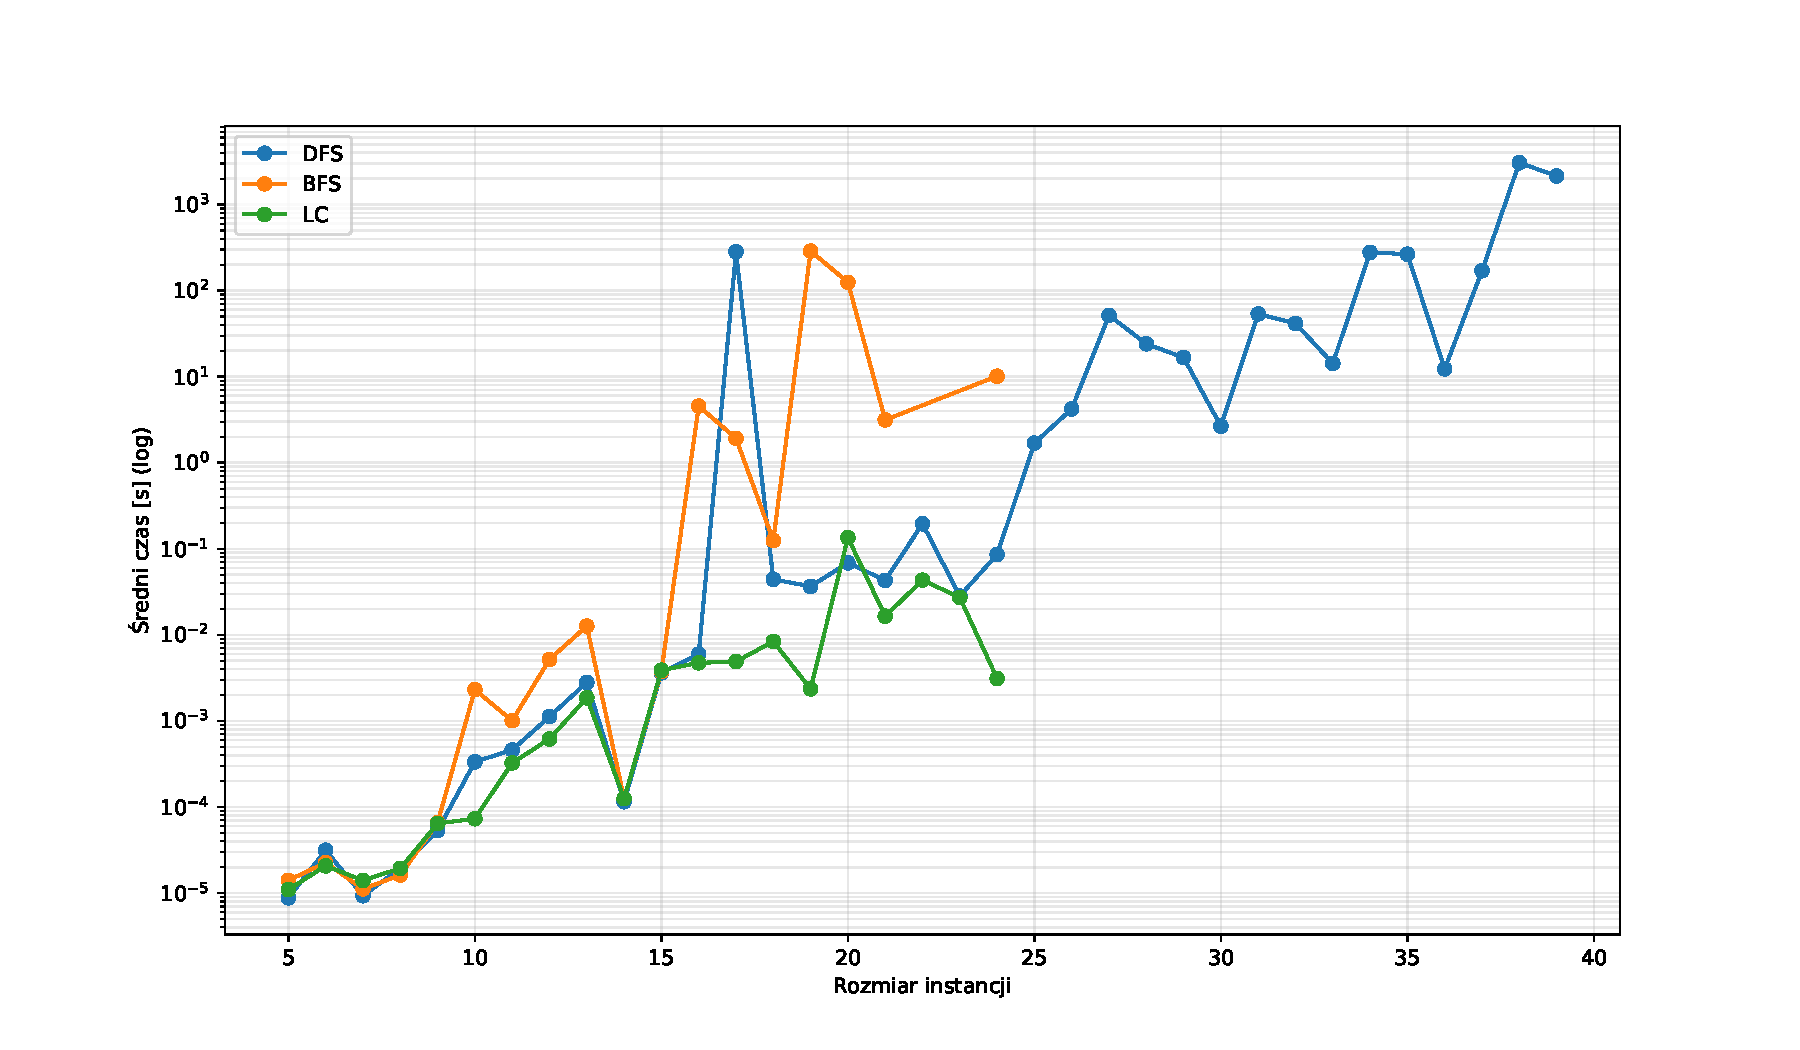
\includegraphics[width=1.0\textwidth]{rys/avg_time_vs_size_log.pdf}
	\caption{Wykres zależności czasu wykonania od rozmiaru instancji $N$ (skala logarytmiczna).}
	\label{fig:wykres_czasu}
\end{figure}
\begin{figure}[H]
	\centering
	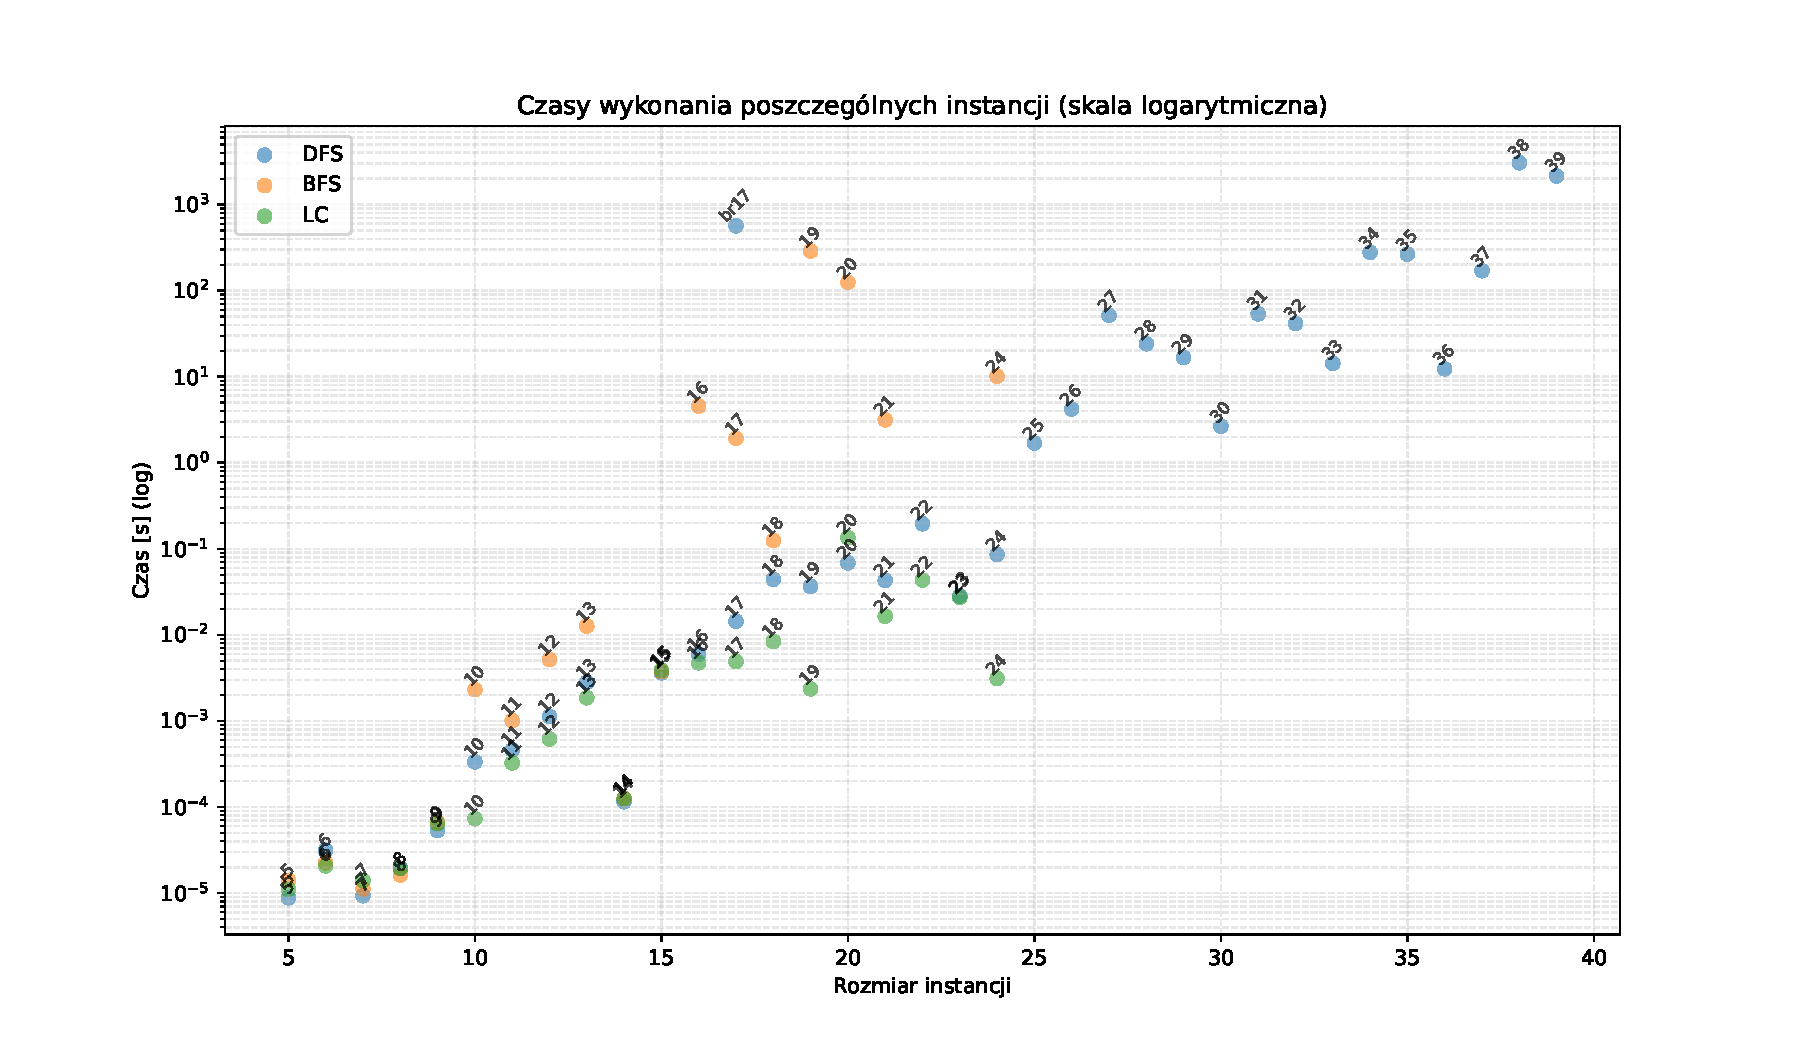
\includegraphics[width=1.0\textwidth]{rys/instance_points_log.pdf}
	\caption{Wykres zależności czasu wykonania od rozmiaru instancji $N$ (skala logarytmiczna).}
	\label{fig:wykres_czasu_instancje}
\end{figure}



Z powyższych wykresów wynika, że nie da się określić złożoności czasowej algorytmów, ponieważ silnie zależy ona od samej instancji, jednakże dla dostępnych danych pomiarowych wyznaczono linie trendu, które prezentuje Tabela~\ref{tab:trendy}

\begin{table}[h]
	\centering
	\caption{Parametry funkcji trendu wykładniczego $t(n) = C \cdot k^n$ dla badanych algorytmów}
	\label{tab:trendy}
	\begin{tabular}{l c c r}
		\toprule
		\textbf{Algorytm} & \textbf{Stała $C$} & \textbf{Wsp. wzrostu $k$} & \textbf{Wzrost \% ($n+1$)} \\ 
		\midrule
		BFS & $3,96 \cdot 10^{-8}$ & $2,554$ & $155,4\%$ \\
		DFS & $1,17 \cdot 10^{-6}$ & $1,723$ & $72,3\%$ \\
		LC  & $1,45 \cdot 10^{-6}$ & $1,561$ & $56,1\%$ \\ 
		\bottomrule
	\end{tabular}
\end{table}



\subsection{Maksymalny rozmiar instancji}
Jednym z wymogów projektu było oszacowanie maksymalnego rozmiaru instancji problemu ATSP, dla której algorytm B\&B jest w stanie znaleźć globalne optimum w rozsądnym czasie oraz przy ograniczeniu dostępnej pamięci RAM. 

Dla algorytmu przeszukiwania w głąb maksymalny rozmiar instancji wyniósł $N=39$, zaś ograniczenie wynikało z przekroczeia czasu obliczeń 30 minut.

Dla aglorytmów przeszukiwania w szerz oraz lowest cost ograniczeniem okazała się ilość dostępnej pamięci RAM, zaś maskymalny rozmiar instancji wynosi $N=24$.

Należy zwrócić uwagę, że maskymalny rozmiar instancji w przypadku tych algorytmów nie jest jedynie zależny od jakości sprżetu. Dodatkowym czynnikiem względem algorytmów badanych w ramach etapu 1 jest rozłożenie kosztów w macierzy kosztów czyli maksymalny rozmiar instancji zależy od samej instancji.

% ---------------------------------------------------------------------------------------------------------------------

\section{Podsumowanie i wnioski końcowe}

Przeprowadzone badania oraz wdrożenie algorytmu Branch and Bound dla asymetrycznego problemu komiwojażera pozwalają na wyciągnięcie kilku kluczowych wniosków dotyczących dynamiki działania różnych strategii przeszukiwania przestrzeni:

\begin{itemize}
	\item \textbf{Skrajna nieefektywność pamięciowa metody BFS i LC:} Przeszukiwanie wszerz nie nadaje się do rozwiązywania problemu ATSP za pomocą B\&B dla instancji większych niż trywialne ($N \ge 15$). Wyznaczenie UB za pomocą RNN słabo odcina ścieżki co powduje, że na stos trafia wiele węzłów szybko wyczerpując dostępną pamięc. Analogicznie wygląda to dla LC, które zależnie od instancji jest niemal identyczne z BFS. Jedyną przwewagą jest znacząca redukcja czasu obliczeń względem BFS.
	
	\item \textbf{Zaskakująca przewaga metody DFS nad Lowest-Cost:} Uzyskane wyniki przeczą intuicyjnemu założeniu, jakoby strategia Best-First (Lowest-Cost), wspierana przez kolejkę priorytetową, była zawsze najszybsza dzięki "inteligentnemu" rozwijaniu najtańszych węzłów. W tym wdrożeniu metoda \textbf{DFS okazała się szybsza oraz pozwala rozwiązywać dwukrotnie większe problemy} 
	\begin{enumerate}
		\item \textit{Struktura danych i narzut obliczeniowy:} Stos w DFS operuje w czasie $O(1)$ na odłożenie i pobranie elementu, podczas gdy kolejka priorytetowa dla Lowest-Cost wymaga logarytmicznego czasu tasowania sterty. Przy milionach odwiedzonych węzłów narzut ten staje się wąskim gardłem.
		\item \textit{Szybkie znalezienie dobrego górnego ograniczenia:} DFS bardzo szybko zagłębia się w drzewo aż do liścia, znajdując kompletny (często całkiem dobry) cykl Hamiltona. Zdobyta w ten sposób "realna" wartość funkcji celu (\textit{upper bound}) pozwala algorytmowi w początkowych fazach działania na niezwykle agresywne i skuteczne odcinanie reszty gałęzi.
	\end{enumerate}
	
	\item \textbf{Porównanie do przeglądu zupełnego (Brute-Force):} W pierwszym etapie projektu ustalono, że metoda \textit{Brute-Force} była w stanie w rozsądnym czasie rozwiązać problem dla zaledwie $N \approx 15$. Dzięki redukcji macierzy (metoda Little'a) i skutecznemu przycinaniu nieskutecznych gałęzi drzewa za pomocą strategii DFS, granicę tę przesunięto do $N \approx 39$.
\end{itemize}

Konkludując, algorytm B\&B jest wysoce potężną metodą dokładną, o ile powiąże się go z odpowiednią, wydajną strukturą przeglądania. Do asymetrycznego problemu komiwojażera w wariancie bazującym na redukcji macierzy, optymalnym wyborem okazuje się być algorytm DFS, łączący mikroskopijny narzut pamięciowy z ogromnym potencjałem wczesnego przycinania przestrzeni rozwiązań.
	
\subsection	{Uwagi implementacyjne}
W implementacji przeszukiwania wszerz można znacząco zwiększyć maksymalny rozmiar instancji kosztem czasu obliczeń poprzez przechowywanie histori operacji na macierzy kosztów zamiast pełnej macierzy redukcji.
\newpage

\section{Środowisko testowe}
W celu zapewnienia powtarzalności wyników oraz rzetelnej analizy wydajności zaimplementowanych algorytmów, wszystkie testy zostały przeprowadzone w ustandaryzowanym środowisku sprzętowo-programowym. Specyfikacja techniczna jednostki obliczeniowej została przedstawiona poniżej:

\subsection{Specyfikacja sprzętowa}
\begin{itemize}
	\item \textbf{Procesor:} AMD Ryzen 7 5800H (8 rdzeni, 16 wątków). Architektura Zen 3 (Cezanne).
	\item \textbf{Pamięć Cache:}
	\begin{itemize}
		\item L1 cache: 512 KiB
		\item L2 cache: 4 MiB
		\item L3 cache: 16 MiB (współdzielona)
	\end{itemize}
	\item \textbf{Pamięć RAM:} 16 GiB DDR4 Synchronous (2 x 8 GiB, praca w trybie Dual-Channel).
	\item \textbf{Dysk:} NVMe SSD Samsung 1024 GB (wykorzystywany do zapisu logów i wyników CSV).
	\item \textbf{Karta graficzna:} NVIDIA GeForce GTX 1650 Mobile / AMD Radeon Vega Series (nieużywane w procesie obliczeń CPU-bound).
\end{itemize}

\subsection{Środowisko programowe}
\begin{itemize}
	\item \textbf{System operacyjny:} Linux (Ubuntu) 
	\item \textbf{Język programowania:} C++23 (Standard ISO/IEC 14882:2023)
	\item \textbf{Kompilator:} GCC/G++ (wykorzystujący optymalizacje poziomu \texttt{-O3})
	\item \textbf{Narzędzia analityczne:} Python 3.x (biblioteki Pandas, Matplotlib) do generowania wykresów i analizy statystycznej.
\end{itemize}	
	
	
	
\end{document}